\documentclass[a4paper]{article}
\usepackage[utf8]{inputenc}
\usepackage[russian]{babel}
\usepackage[T2]{fontenc}
\usepackage[warn]{mathtext}
\usepackage{graphicx}
\usepackage{amsmath}
\usepackage{floatflt}
\usepackage[left=20mm, top=20mm, right=20mm, bottom=20mm, footskip=10mm]{geometry}


\graphicspath{ {images/} }
\usepackage{multicol}
\setlength{\columnsep}{2cm}


\begin{document}

\begin{titlepage}
	\centering
	\vspace{5cm}
	{\scshape\LARGE Московский физико-технический институт \par}
	\vspace{5cm}

	{\huge\bfseries Масс-спектроскопия остаточных газов \par}
	\vspace{0.5cm}
	{\huge\bfseries Квадрупольный масс-анализатор \par}
	\vspace{1cm}
	{\scshape\Large Лабораторная работа по курсу <<Вакуумная электроника>>\par}
	\vspace{1cm}
	\vfill
\begin{flushright}
	{\large выполнила студентка 653 группы ФФКЭ}\par
	\vspace{0.3cm}
	{\LARGE Карпова Татьяна Кирилловна} \par

	
\end{flushright}
	

	\vfill

% Bottom of the page
	Долгопрудный, 2018 г.
\end{titlepage}

\section{Цель работы}
\begin{enumerate}
    \item Исследовать масс-спектр остаточных газов в вакуумной установке
\item Напустить в вакуумный объем аргон и исследовать масс-спектр образовавшейся газовой смеси.
\item В полученных масс-спектрах идентифицировать максимальное количество пиков
(расшифровать спектры).
\end{enumerate}

\section{Теоретические положения}

Масс-спектрометрия – метод исследования пробы вещества, основанный на ионизации атомов и молекул, входящих в состав пробы. Масс-спектрометрия измеряет массу иона, или, точнее, отношение массы иона к его
заряду - $m/Z$ ($m$ – масса иона, измеренная в атомных единицах массы – а.е.м.; $Z$ – заряд иона, измеренный в
элементарных зарядах $Z = Q/e $) Анализ вещества происходит по следующим этапам:
\begin{enumerate}
    \item Превращение нейтральных частиц – атомов или молекул в заряженные частицы – ионы;
    \item Разделение образовавшихся ионов в пространстве в соответствии с их отношением $m/Z$.
    \item Измерение интенсивности пучка направленно движущихся ионов с определенным отношением $m/Z$.
\end{enumerate}

Зависимость количества ионов от величины $m/Z$ представленная в виде графика или таблицы,
называется масс-спектром вещества. Приборы, в которых регистрация ионов осуществляется
электрофизическими методами, называются масс-спектрометрами, а приборы с регистрацией ионов на
фотопластинках - масс-спектрографами. \par
Масс-спектрометр работает в условиях достаточно высокого вакуума ($10^-^5$ – $10^-6$ Торр и выше). Создать вакуум необходимо для уменьшения рассеяния ионного пучка на молекулах остаточных газов, иначе ухудшается разрешающая способность масс-спектрометра. \par
Масс-спектрометры характеризуются разрешающей способностью и чувствительностью.

\begin{figure}[h]
\begin{center}
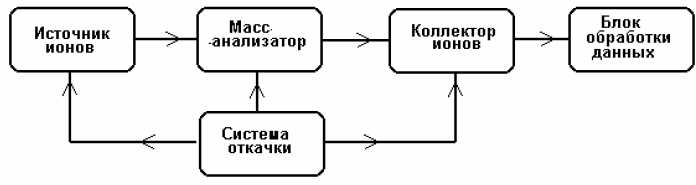
\includegraphics[width=10cm]{fig1.PNG}
\caption{Блок-схема масс-спектрометра}
\label{ris:experimoriginal} %% метка рисунка для ссылки на него

\end{center}
\end{figure}

В работе используется квадрупольный масс-спектрометр. Квадрупольный масс-анализатор относится к анализаторам с динамическим принципом действия. Он представляет собой квадрупольный конденсатор (рис. 2), состоящий из четырех параллельных, симметрично расположенных проводящих стержней. К парам параллельных стержней приложены постоянное напряжение $U_0$ и переменное высокочастотное $U\omega \cos(\omega t)$ ($\omega$ – частота, $t$ – время); их суммы для каждой пары равны по величине и противоположны по знаку. \par

Действие такого анализатора состоит в том, что ионы, влетевшие в анализатор, движутся в камере анализатора вдоль оси 0z, параллельной продольным осям стержней, по сложным объемным спиралевидным траекториям, совершая поперечные колебания вдоль осей x и y. При фиксированных значениях частоты и амплитуды переменного напряжения ионы с определенными значениями $m/Z$ проходят через квадрупольный конденсатор и попадают на коллектор; у ионов с другими значениями $m/Z$ амплитуда поперечных колебаний достигает такой величины, что они ударяются о стержни и разряжаются на них. \par Сканирование масс-спектра производится путем изменения постоянного и переменного напряжения (или частоты генератора). Для современных квадрупольных масс-спектрометров разрешающая способность достигает значения R=10000.

\begin{figure}[h]
\begin{center}
\begin{minipage}[h]{0.4\linewidth}
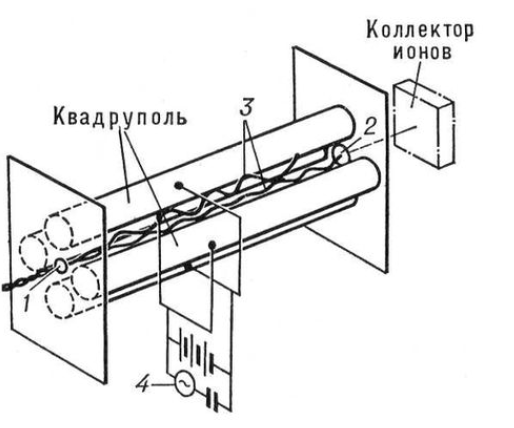
\includegraphics[width=1\linewidth]{quadrup.PNG}
\caption{Устройство квадрупольного масс-спектрометра } %% подпись к рисунку\label{ris:experimoriginal} %% метка рисунка для ссылки на него
\end{minipage}
\hfill 
\begin{minipage}[h]{0.7\linewidth}
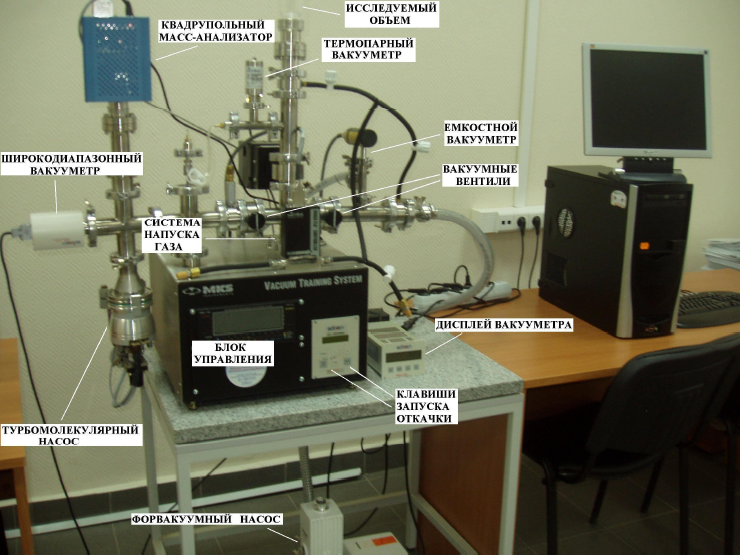
\includegraphics[width=1\linewidth]{fig3.PNG}
\caption{Внешний вид лабораторной установки }
\label{ris:experimcoded}
\end{minipage}
\end{center}
\end{figure}



\section{Ход работы}

\begin{enumerate}
    \item Откачаем вакуумную установку до давления порядка $10^-^2$ Торр. Далее, изменяя значение натекания, будем анализировать состав смеси остаточных газов в зависимости от давления. Графики приведены на рисунках 
    
    
    


\newpage

\item Проанализируем полученные данные. Видим, что при увеличении натекания и, соответственно, при повышении давления в вакуумной установке состав остаточных газов становится всё более разнообразным. Если при малом давлении (0.1 Торр) чётко прослеживаются только кислород (16 аем), вода и ОН-группа, то при увеличении давления до 0.7 Торр появляются такие газы как азот (14 аем), молекулярный азот и кислород с большими массами. Ниже приведена таблица соответствия веществ и их атомных единиц массы

        \begin{table}[h]
    \centering
    \begin{center}
    \caption{Остаточные газы и их атомные единицы массы}
    \end{center}
    \vspace{0.1cm}
    \label{tab:my_label}
    \begin{tabular}{ |p{4cm}||p{2cm}|p{2cm}|}
 \hline
 Название вещества & Формула & а.е.м. \\
 \hline
 \hline
Азот  & $N$ & 14 \\
   \hline
Кислород  & $O$ & 16 \\
   \hline
  ОН-группа & $OH^-$ & 17 \\
   \hline
Вода  & $H_2 O$ & 18 \\

   \hline
Молекулярный кислород  & $O_2$ & 28\\
   \hline
Молекулярный азот  & $N_2$ & 32\\
\hline
 
\end{tabular}
\end{table}

\item Далее подсоединим к вакуумной установке баллон с аргоном и с помощью натекателя перенесём исследуемый газ к камере масс-спектрографа. Исследуем графики парциальных давления газов в этом случае. К сожалению, из-за неисправности натекателя не удаётся подать к анализатору чистый газ, поэтому результаты измерения парциальных давлений не отличаются от измеренных ранее в процентном соотношении.

\vspace{20cm}
\vspace{10cm}

\begin{figure}[h]
\begin{center}
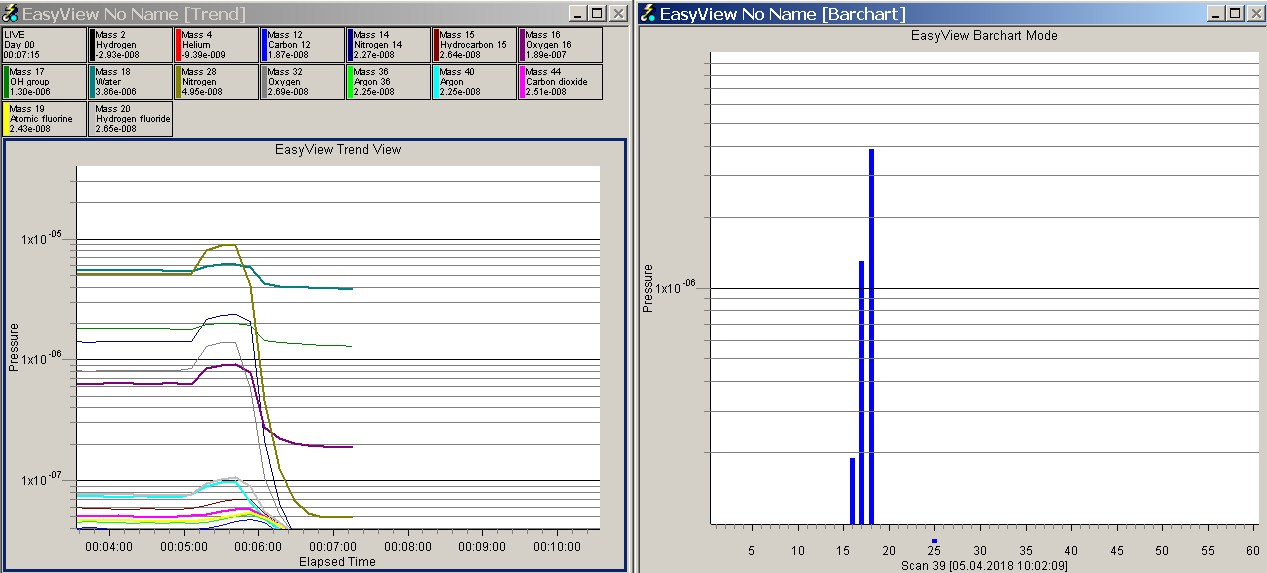
\includegraphics[width=16cm]{gas_3.jpg}
\caption{Распределение парциальных давлений после присоединения баллона с аргоном}
\label{ris:experimoriginal} %% метка рисунка для ссылки на него

\end{center}
\end{figure}


\end{enumerate}

\section{Вывод}
\begin{enumerate}
    \item Был исследован принцип работы квадрупольного масс-анализатора;
    \item В ходе работы был изучен полученный масс-спектр остаточных газов в вакуумной установке с помощью квадрупольного масс-анализатора;
    \item При напускании в вакуумный объем газ из баллона, получен масс-спектр газовой смеси. По этим спектрам видно, что исследуемый газ (аргон) после прохождения к анализатору смешивается с другими газами, и смесь становится схожей составу с воздухом (связано это либо с неисправностью натекателя, либо с малым остатком заявленного газа в баллоне).
\end{enumerate}

\begin{figure}[h]
\begin{center}
\begin{minipage}[h]{0.5\linewidth}
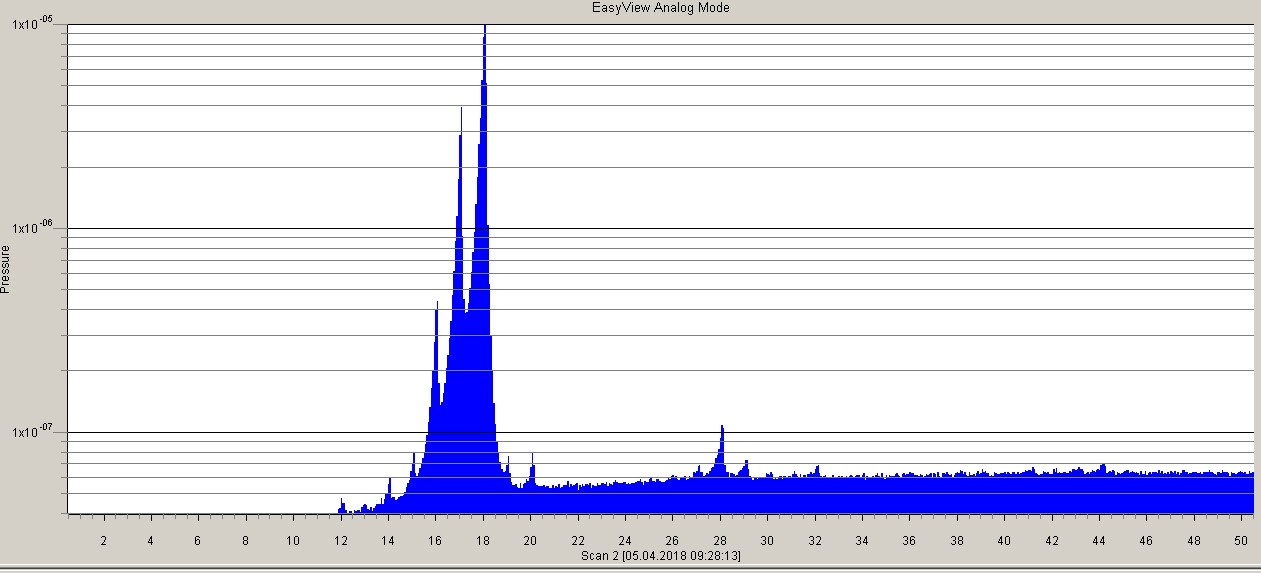
\includegraphics[width=1\linewidth]{flow1,5analog.jpg}
\caption{Парциальные давления газов при натекании 1.5 sccm и давлении 0.1 Торр, аналоговый график  } %% подпись к рисунку\label{ris:experimoriginal} %% метка рисунка для ссылки на него
\end{minipage}
\hfill 
\begin{minipage}[h]{0.4\linewidth}
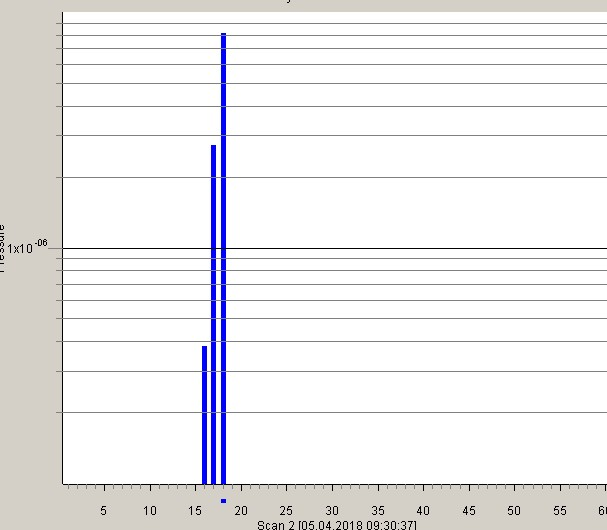
\includegraphics[width=1\linewidth]{flow2gisto.jpg}
\caption{Парциальные давления газов при натекании 1.5 sccm и давлении 0.1 Торр, гистограмма  }
\label{ris:experimcoded}
\end{minipage}
\end{center}
\end{figure}

\begin{figure}[h]
\begin{center}
\begin{minipage}[h]{0.5\linewidth}
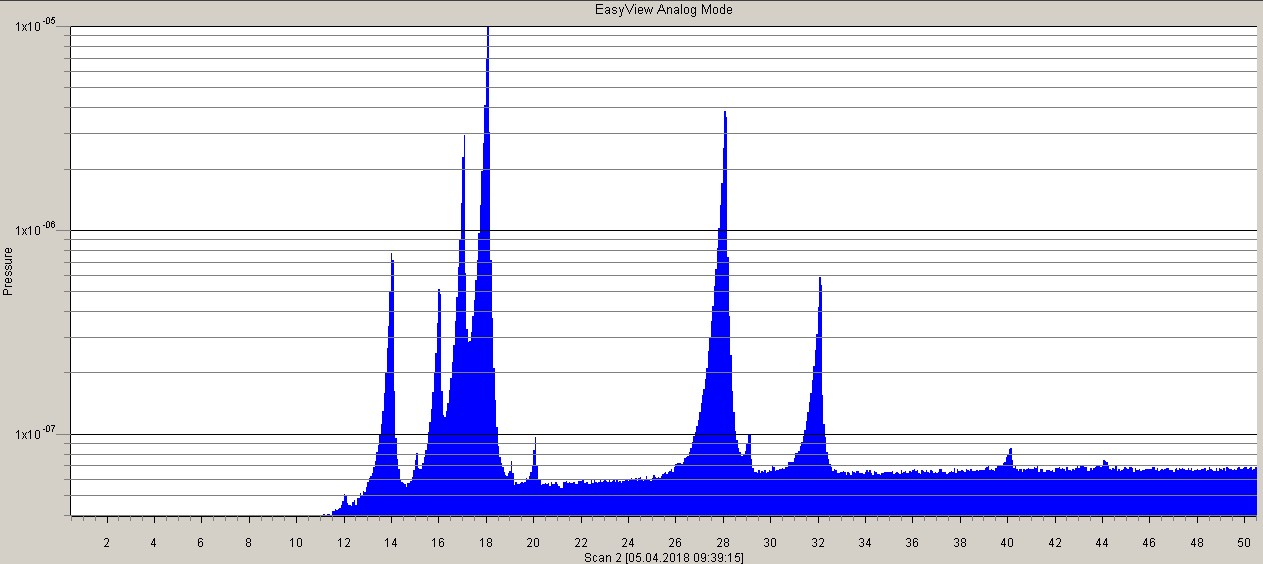
\includegraphics[width=1\linewidth]{flow12analog.jpg}
\caption{Парциальные давления газов при натекании 12 sccm и давлении 0.3 Торр, аналоговый график  } %% подпись к рисунку\label{ris:experimoriginal} %% метка рисунка для ссылки на него
\end{minipage}
\hfill 
\begin{minipage}[h]{0.4\linewidth}
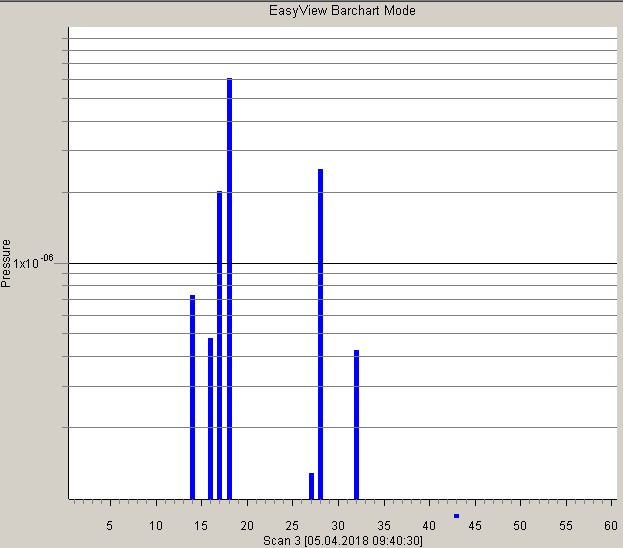
\includegraphics[width=1\linewidth]{flow12gisto.jpg}
\caption{Парциальные давления газов при натекании 12 sccm и давлении 0.3 Торр, гистограмма  }
\label{ris:experimcoded}
\end{minipage}
\end{center}
\end{figure}

\begin{figure}[h]
\begin{center}
\begin{minipage}[h]{0.5\linewidth}
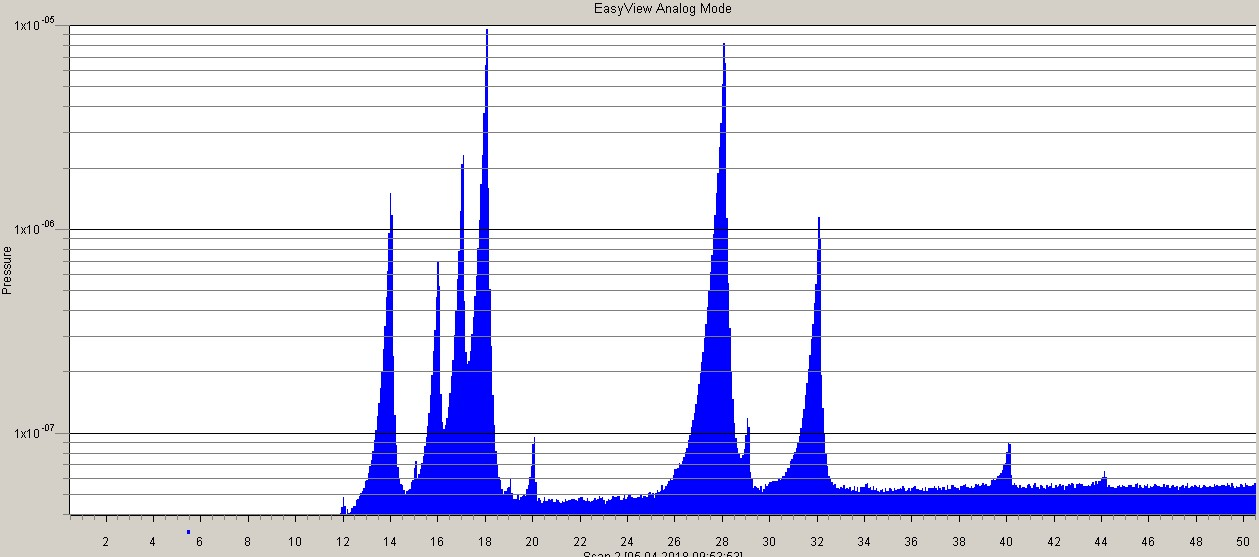
\includegraphics[width=1\linewidth]{flow28analog.jpg}
\caption{Парциальные давления газов при натекании 28 sccm и давлении 0.7 Торр, аналоговый график  } %% подпись к рисунку\label{ris:experimoriginal} %% метка рисунка для ссылки на него
\end{minipage}
\hfill 
\begin{minipage}[h]{0.4\linewidth}
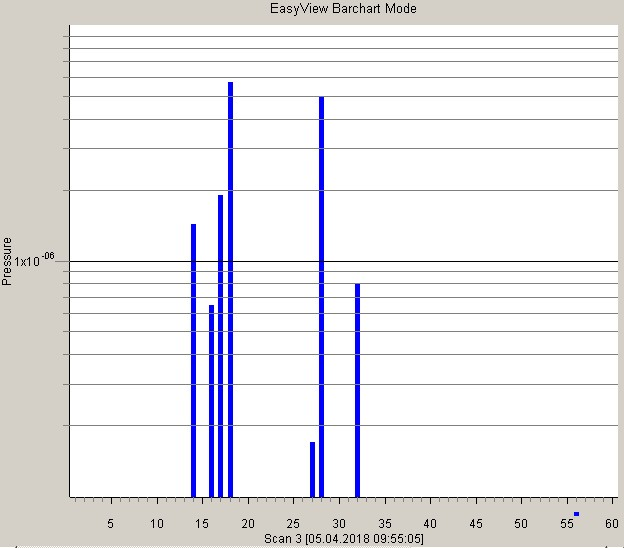
\includegraphics[width=1\linewidth]{flow28gisto.jpg}
\caption{Парциальные давления газов при натекании 28 sccm и давлении 0.7 Торр, гистограмма  }
\label{ris:experimcoded}
\end{minipage}
\end{center}
\end{figure}


\end{document}
